\newpage
\setcounter{section}{0}
\renewcommand{\thesection}{\arabic{section}}

\begin{center}
    \Huge
    \textbf{Modul 1}
    
    Wireless Connection

\end{center}

\section{pendahuluan}

Pada Wireless Jaringan Komputer, terdapat setidaknya 3 jenis, yaitu Point-to-Point Protocol
(PPP), Point-to-multipoint dan Wireless Bridging.

Point-to-Point Protocol (PPP) adalah data link protokol yang umum digunakan dalam
membangun hubungan langsung antara dua node jaringan. Hal ini dapat menyediakan koneksi
otentikasi, transmisi enkripsi (menggunakan ECP, RFC 1968), dan kompresi. Jenis ini
biasanya digunakan untuk menghubungkan jaringan antar 2 gedung atau antar 2 BTS (Base
Transceiver Station).

Point-to-multipoint adalah pendekatan yang paling populer untuk komunikasi nirkabel yang
memiliki banyak node, tujuan akhir atau pengguna akhir. Jenis ini biasanya digunakan untuk
membuat wifi atau hotspot yang berasal dari 1 sumber disebar ke banyak client dalam suatu
jaringan.

Wireless Bridging digunakan untuk menghubungkan dua segmen LAN melalui tautan
nirkabel. Kedua segmen akan berada di subnet yang sama dan terlihat seperti dua switch
Ethernet yang dihubungkan oleh kabel ke semua komputer di subnet.

Untuk mengembangkan jaringan komputer berbasis wireless yang berkualitas dan mempunyai
ketersediaan tinggi, penggunaan 3 jenis ini perlu disesuaikan dengan kebutuhan dan kondisi
nya, sehingga kali ini saya akan membahasnya 1 persatu dari 3 jenis koneksi wireless
tersebut.

\section{Tujuan Praktikum}

mengetahui dan memahami 3 jenis koneksi pada jaringan Wireless

\section{Alat dan Bahan}

Berikut adalah alat dan bahan yang digunakan untuk praktikum :

\begin{enumerate}
    \item 2 Router Mikrotik dengan support Wireless
    \item 2 Laptop
    \item 2 Kabel LAN 
    \item Aplikasi Winbox
\end{enumerate}

\section{Topologi}

berikut adalah topologi yang digunakan :

\begin{center}
    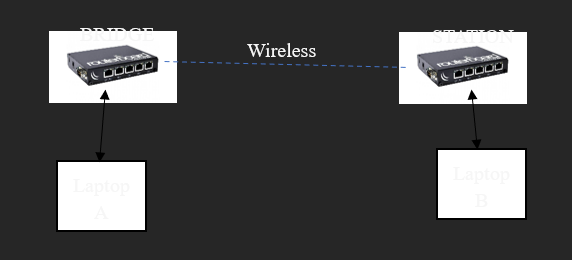
\includegraphics[width=0.7\textwidth]{image/P1/Topologi.png}    
    
    figure.1 Topologi
\end{center}

\section{Langkah Percobaan}
\begin{enumerate}
    \item Persiapan Awal
    
    \begin{enumerate}
        \item Sambungkan PC dan Router mikrotik sesuai dengan topologi
        \item Matikan Firewall pada Laptop
        \item Masuk ke aplikasi Winbox
        \item Pada bagian Neighbour, check apakah ada IP 0000 identity mikrotik
        \item Reset mikrotik ke 0000
        \item Lalu tekan connect
        
        \begin{center}
            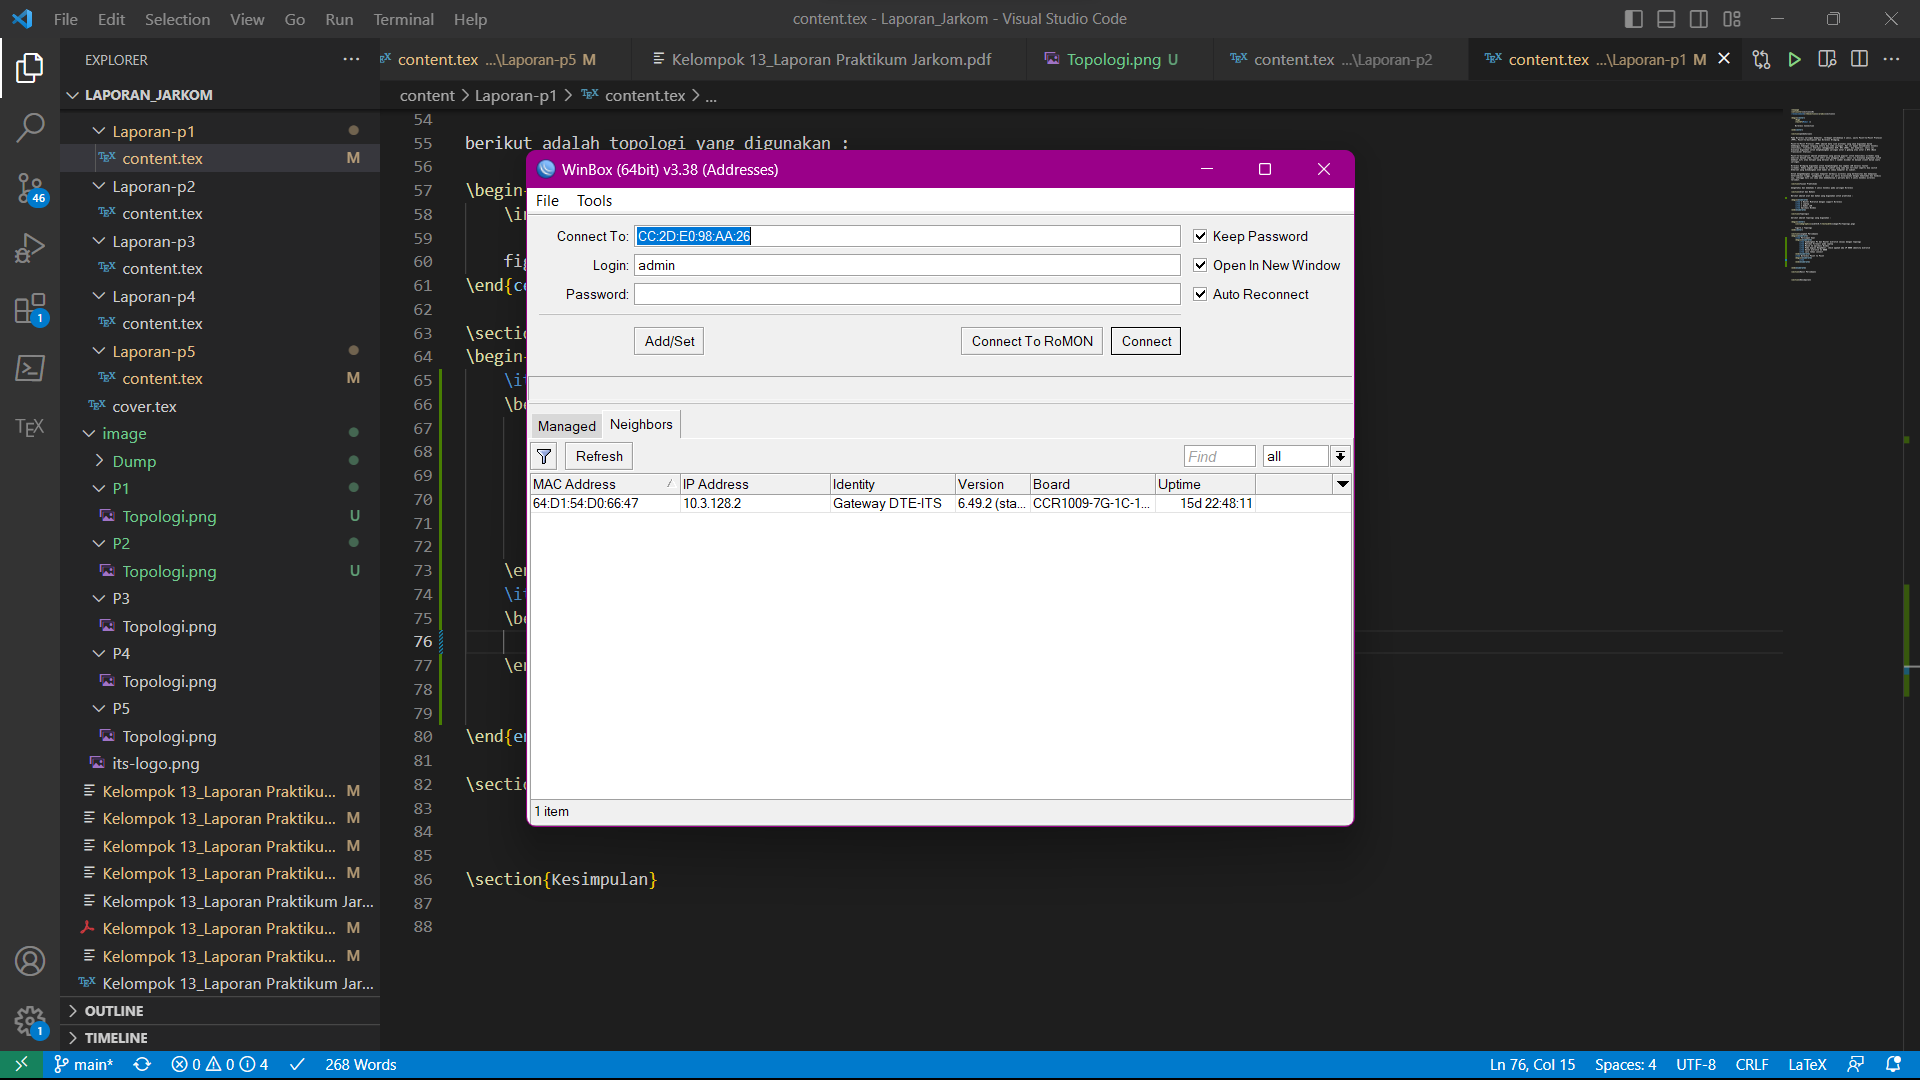
\includegraphics[width=0.7\textwidth]{image/Winbox-interface.png}    
            
            figure.1 Topologi
        \end{center}

    \end{enumerate}

    \item Wireless Point to Point
    
    \begin{enumerate}
        \item 
    \end{enumerate}

    \item Wireless Point to Multipoint
    
    \begin{enumerate}
        \item 
    \end{enumerate}

    \item Wireless Bridging
    
    \begin{enumerate}
        \item 
    \end{enumerate}
    
\end{enumerate}

\section{Hasil Percobaan}



\section{Kesimpulan}

Jaringan Komputer berbasis Wireless dapat menggunakan Teknologi Point to Point, Point to Multipoint dan Wireless Bridging